\documentclass[10pt,letterpaper]{article}
\usepackage[margin=0.9in]{geometry}
\usepackage[OT1]{fontenc}
\usepackage[utf8]{inputenc}
\usepackage{amsmath,amssymb}
\usepackage{booktabs}
\usepackage{array}
\usepackage{graphicx}
\usepackage[font=small,labelfont=bf,labelsep=period,skip=4pt]{caption}
\usepackage{enumitem}
\usepackage[expansion=false]{microtype}
\usepackage[hidelinks]{hyperref}
\usepackage{float}
\usepackage{multicol}
\usepackage{longtable}
\setlength{\parskip}{3pt}
\setlength{\parindent}{0pt}
\setlist{nosep,leftmargin=1.2em}
\setlist[itemize]{label=$\bullet$}
\graphicspath{{../../../plots/a6_generalization/}}
\renewcommand{\arraystretch}{1.05}
\captionsetup[table]{position=above,skip=3pt}
\newcommand{\lead}[1]{\textbf{#1}}
\newcommand{\LL}{L}

\title{\vspace{-2em}CS 312 Assignment 6 writeup}
\author{Sandra Yang}
\date{November 19, 2026}

\begin{document}
\maketitle

\section*{Setup}

\lead{Data and model.} Every run uses the released DNA pool: 30,000 training chunks of 1,024 tokens (a BOS prefix plus 1,023 payload tokens, 30.72M tokens per pass) and a disjoint 1,000-chunk validation set, with a 19-token vocabulary. The model is d8 (8 blocks, width 512, QK normalization, 30.4M parameters). The recipe is AdamW $\beta=(0.9,0.95)$, peak LR $0.003$, WD $3.2$, batch 64 sequences in 8 microbatches, clipping at 1, 4,800 sequences of warmup, then linear decay to zero; 32 passes over the pool (983M tokens of exposure, 15,000 updates). $L$ is the validation NLL in nats per token at the end of training. The fine-tuning parts use 1, 4 or 16 passes. We select and report on the same validation set, so every number below is slightly optimistic.

\lead{Supplied runs and our runs.} The release \texttt{a6-generalization-v1} (W\&B project \texttt{hashimoto-group/public-alchemy-a6}, 48 runs) covers the tuned dense suite d4 to d10 (1a), the 16-epoch LR$\times$WD grid (2a-i), the two 32-epoch AdamW controls (2a-ii), five no-dropout ensemble members (2b-ii), the schedule horizons (3a) and the batch sweep with sharpness probes (3b). We did not retrain any of it. Everything else is our own: we train with the starter \texttt{training.py} on Modal H100/H200 GPUs, final checkpoints and histories under \texttt{a6/<name>} on our volume. Run names are listed at the end.

\lead{Time budget.} The report was written in the 16 hours before the deadline. We queued 77 runs in priority order on two to four GPUs (the class workspace was at its GPU cap); full 32-pass runs take about 50 minutes, fine-tuning runs 2 to 25 minutes. Runs that did not finish are marked as such; the P1(d) and P3(d) explorations and most second seeds were cut, and we say so where it matters.

\lead{Notation and noise.} $\Delta L$ is a loss difference. The supplied d8 ensemble members (seeds 42 to 46, same data order) span 1.2600 to 1.2640, so one-seed differences below about $0.003$ are noise, $0.005$ to $0.02$ are small but real, and $0.03$ or more is a change of regime. Our own second seed of the baseline is reported in Problem 2 where available.

%=====================================================================
\section*{Problem 1. Architecture}

\subsection*{Part (a). Parameter scaling on the supplied suite}

The supplied suite tunes LR, WD and epoch count per size on the same 30k pool (seed 42, Table~\ref{tab:p1}, Figure~\ref{fig:p1}). We fit $L(N)=L_\infty+AN^{-\alpha}$ to the seven selected points.

\begin{figure}[H]\centering
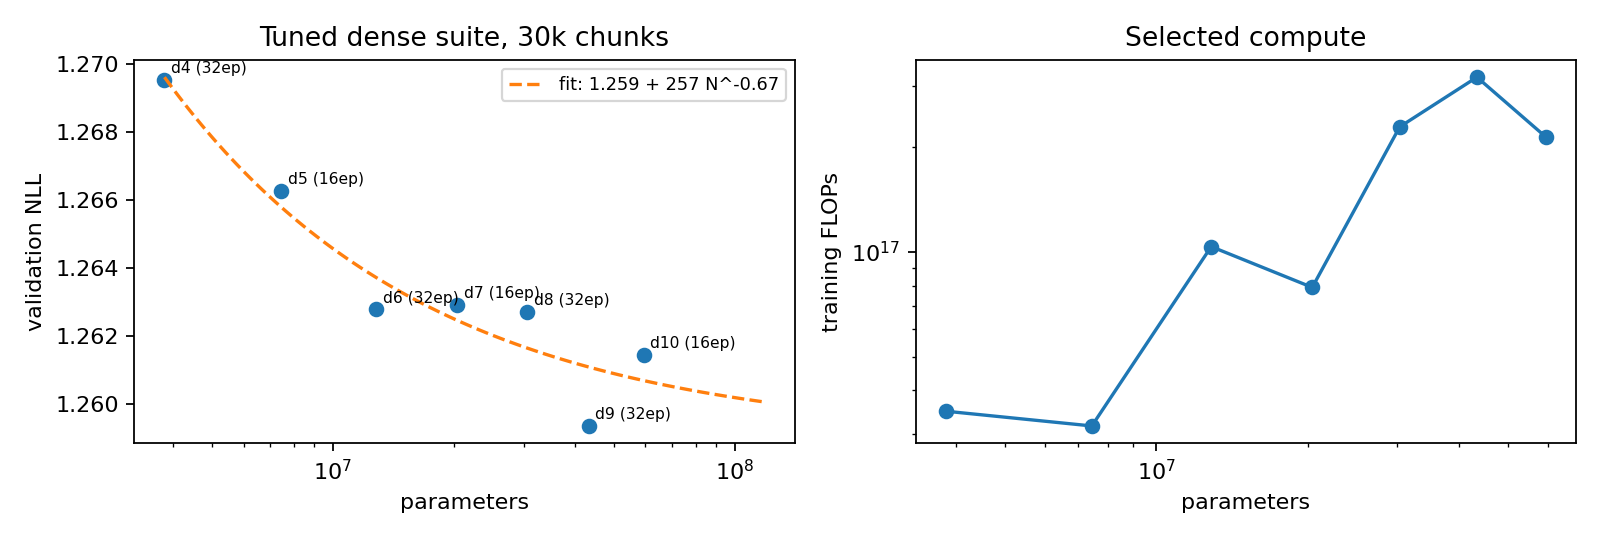
\includegraphics[width=.95\linewidth]{p1_parameters}
\caption{Left: validation NLL of the tuned dense suite against parameter count with the power-law fit (dashed). Right: training FLOPs of the selected recipe at each size.}
\label{fig:p1}
\end{figure}

\begin{table}[H]\centering\small\caption{Problem 1(a): the supplied tuned dense suite (seed 42, linear decay). LR, WD and epochs were selected on validation data per size.}\label{tab:p1}
\begin{tabular}{lrrrrrrr}\toprule Model & width & params (M) & LR & WD & epochs & PFLOP & val NLL \\ \midrule
d4 & 256 & 3.8 & 0.003 & 1 & 32 & 35 & 1.2695 \\
d5 & 320 & 7.4 & 0.003 & 0.8 & 16 & 32 & 1.2663 \\
d6 & 384 & 12.8 & 0.003 & 3.2 & 32 & 104 & 1.2628 \\
d7 & 448 & 20.4 & 0.003 & 1.6 & 16 & 79 & 1.2629 \\
d8 & 512 & 30.4 & 0.003 & 3.2 & 32 & 229 & 1.2627 \\
d9 & 576 & 43.3 & 0.003 & 1 & 32 & 318 & 1.2594 \\
d10 & 640 & 59.4 & 0.003 & 1 & 16 & 214 & 1.2614 \\
\bottomrule\end{tabular}\end{table}


\begin{itemize}
\item \lead{Fit.} $L(N)=1.2590+257\,N^{-0.67}$ with $N$ in parameters, equivalently $1.2590 + 0.026\,(N/10^6)^{-0.67}$. The fitted floor sits only $0.003$ below the best measured point, and the whole suite spans $0.010$ nats (1.2695 at d4 to 1.2594 at d9).
\item \lead{Not monotonic.} d6, d7 and d8 are within $0.0002$ of each other (1.2628, 1.2629, 1.2627), and d10 (1.2614) is worse than d9 (1.2594). With one seed and $0.003$ of seed noise, the suite is consistent with a flat region from 13M to 60M parameters. Returns diminish sharply: going 4$\times$ from d4 to d6 buys $0.007$, going 4.6$\times$ from d6 to d10 buys $0.001$.
\item \lead{Epochs and compute.} The selected epoch count alternates between 16 and 32 (d5, d7, d10 pick 16), with no trend toward fewer passes at larger size; the 64-pass d8 reference (1.2691) is worse than 8 passes (1.2687), so 32 passes is already past the optimum for d8 and the selected WD rises with size up to d8 (1.0, 0.8, 3.2, 1.6, 3.2) then drops to 1.0 for d9/d10. Training compute therefore grows roughly linearly in $N$ with a factor-of-two sawtooth from the epoch choice (Figure~\ref{fig:p1}, right).
\item \lead{Reading.} At 30k chunks the data, not the parameter count, limits the loss: a 15$\times$ increase in parameters moves $L$ by less than one ensemble-member's worth of seed noise times three. The remaining problems ask how to move $L$ by changing what we do with the same 30k chunks.
\end{itemize}

\subsection*{Parts (b, c). MoE and looping from Assignment 5}

\lead{MoE and looping at matched data.} We retrained the two A5 architectures on the DNA pool: a 4-expert learned top-1 MoE with quantile balancing (about four times the FFN parameters of d8, the same active compute) and a looped model (prelude, a shared block applied 6 times with RMS normalization and recall, coda; fewer parameters than d8). Table~\ref{tab:p1ours} lists the results; the LR .01 and .001 trials sit at the end of the queue and are marked cut where unfinished.
\begin{itemize}
\item Neither beats dense. At LR .003 the MoE reaches 1.2656 (+0.003 over d8) and the loop 1.2693 (+0.007). The MoE tracks our dense runs through pass 24 (1.2753 against 1.2754 for dropout .05) and then gains less during the final LR decay, consistent with the extra capacity fitting the repeated 30k chunks rather than new structure.
\item This reverses the A5 ordering, where the MoE won clearly on fresh text. On 30k repeated DNA chunks the supplied suite is already flat above d6, so more parameters (MoE) buy nothing and fewer (loop) cost a little; the data, not the architecture, sets the floor.
\item Prediction we make for Part (d): any architecture change that only adds capacity will land within $\pm0.005$ of d8 here; only changes that act as regularizers (dropout, ensembles) move the number.
\end{itemize}


\begin{table}[H]\centering\small\caption{Problems 1(b,c): A5 architectures retrained on the 30k pool for 32 passes at WD 3.2, three LRs, seed 42, data order paired with the supplied baseline. Unfinished cells are marked.}\label{tab:p1ours}
\begin{tabular}{lrrrrr}\toprule Architecture & LR .001 & LR .003 & LR .01 & best & $\Delta L$ vs d8 \\ \midrule
MoE, 4 experts, learned top-1, quantile balance & -- & 1.2656 & -- & 1.2656 & +0.0029 \\
Loop, prelude + 6 passes of a shared block + coda, RMS + recall & -- & 1.2693 & -- & 1.2693 & +0.0066 \\
Dense d8 (supplied) & -- & 1.2627 & -- & 1.2627 & 0 \\
\bottomrule\end{tabular}\end{table}


%=====================================================================
\section*{Problem 2. Regularization}

\subsection*{Part (a). Weight decay}

\lead{(i) LR$\times$WD on the supplied 16-epoch grid.} The grid has 21 completed runs (LR $\in\{.001,.003,.01\}$, WD $\in\{0,.1,.3,1,3.2,10,30\}$). Figure~\ref{fig:lrwd} shows the quadratic fit in $\log$LR and $\log$WD (positive WD only, RMSE $0.0086$) and the measured losses against the product.

\begin{figure}[H]\centering
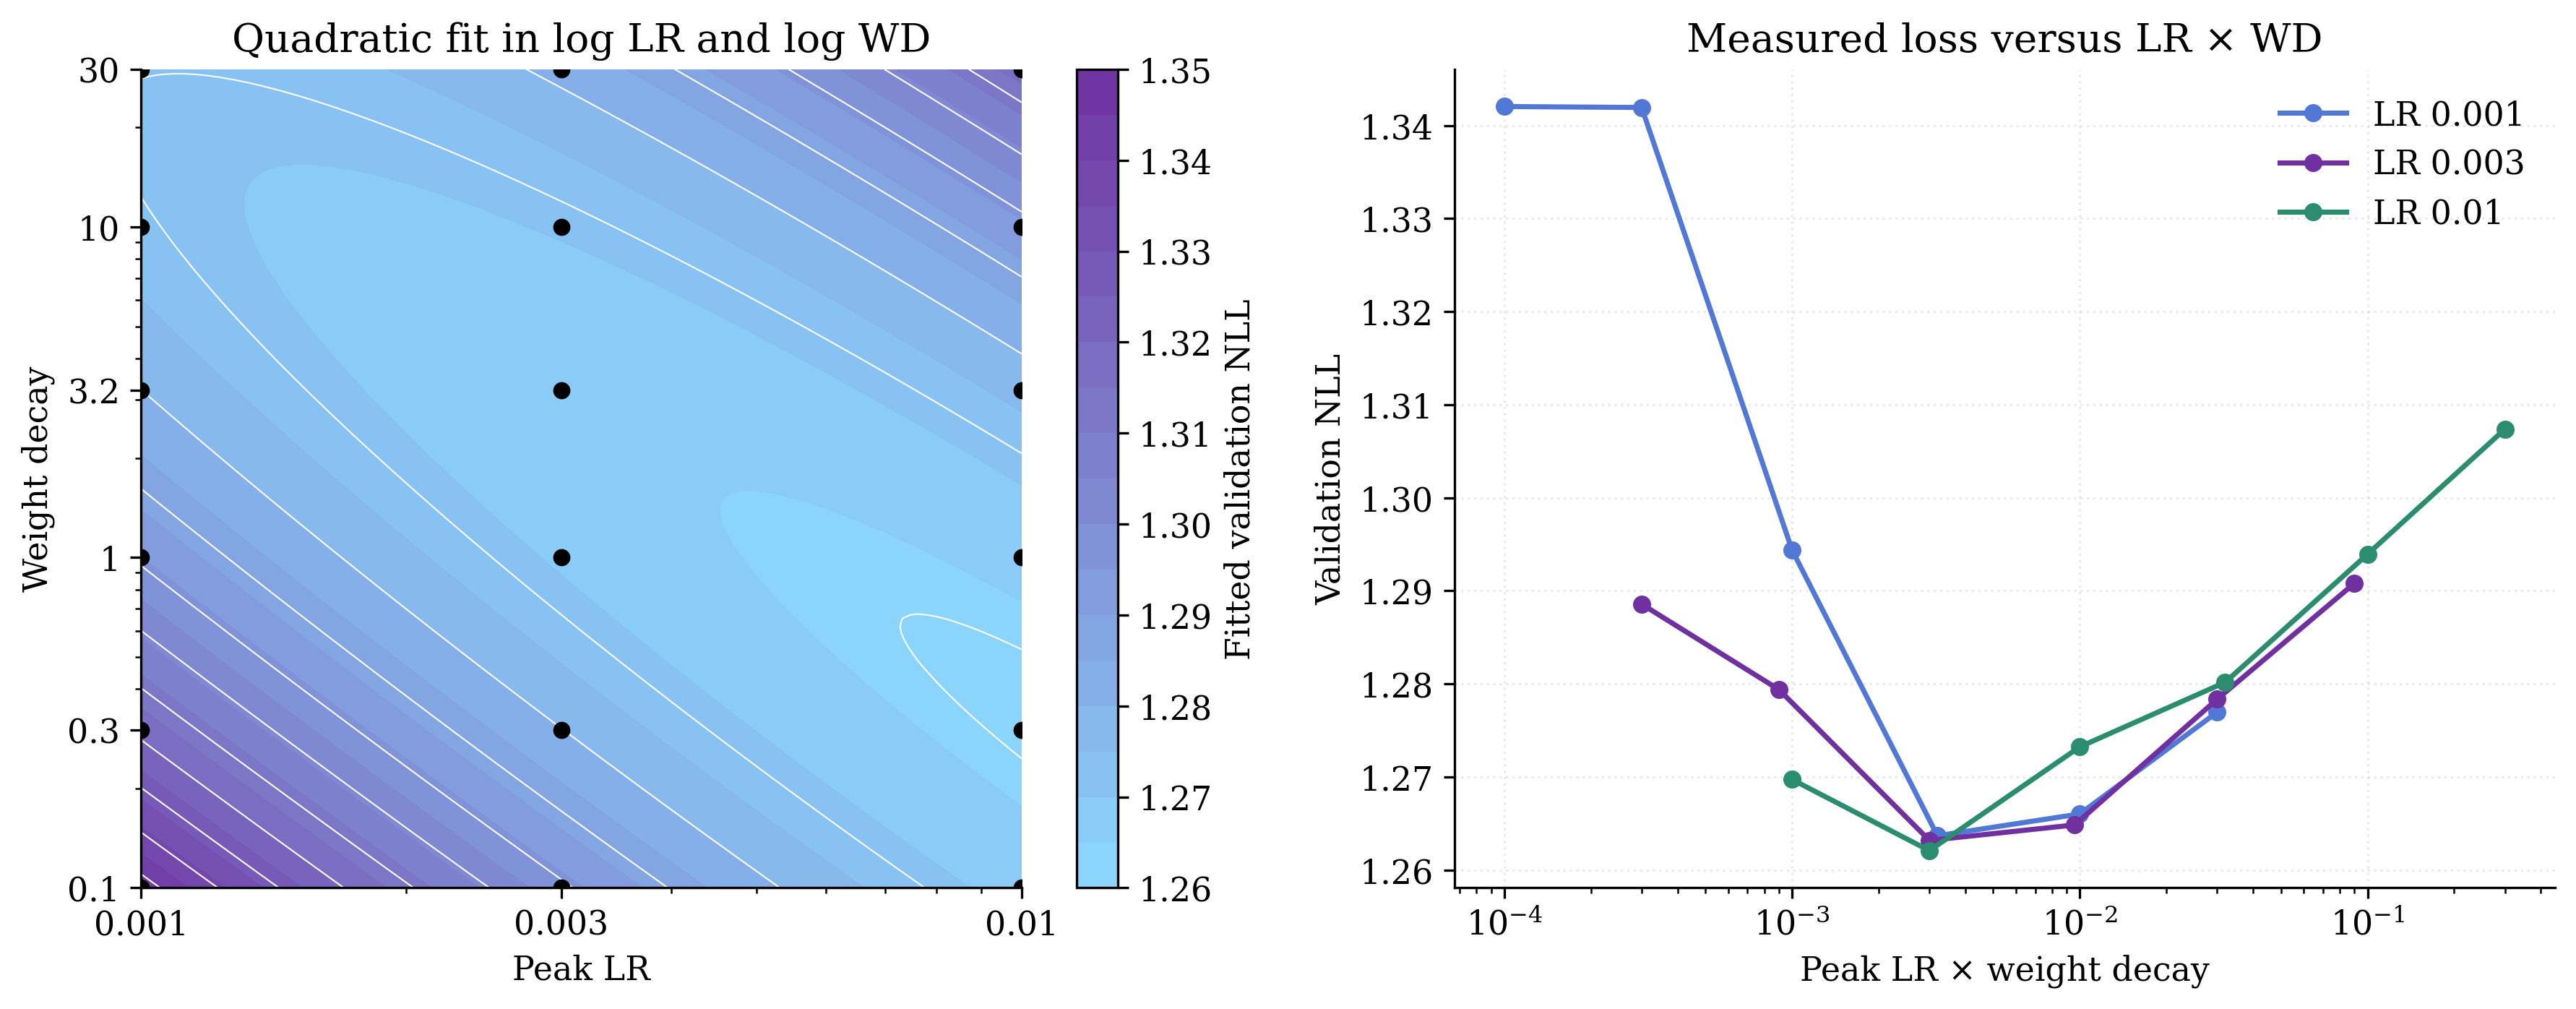
\includegraphics[width=.95\linewidth]{lr_wd}
\caption{Left: quadratic fit of validation NLL in $\log$ LR and $\log$ WD at 16 passes (dots are the grid). Right: measured loss against LR$\times$WD, one line per LR.}
\label{fig:lrwd}
\end{figure}

\begin{itemize}
\item \lead{The product organizes the grid.} All three LR lines reach their minimum at LR$\times$WD $=0.003$ (LR .01/WD .3 at 1.2621, LR .003/WD 1 at 1.2632, LR .001/WD 3.2 at 1.2637) and agree within $0.004$ to the right of it. To the left, the lines separate: LR .001 at small WD is $0.05$ worse than LR .01 at the same product, so the product predicts the loss once the LR is at least $0.003$ and otherwise sets a lower bound.
\item \lead{How much more WD.} At LR .003 the best WD in the 16-pass grid is $1$ (1.2632 against 1.2886 at WD .1, a $0.025$ gap), 10$\times$ the earlier reference. At 32 passes the course selection moved to WD 3.2 (32$\times$), consistent with a product rule plus a longer run: the decay time constant $1/(\eta\lambda)$ should stay a fixed fraction of training.
\item \lead{Quadratic fit.} The fitted surface puts its minimum on the LR .01 edge at WD near $0.4$; the surface is a valley along the product line rather than a bowl, so a quadratic in two variables is a coarse summary and the $0.0086$ RMSE is comparable to the differences between good points.
\end{itemize}

\lead{(ii) Hyperball against AdamW.} The supplied 32-pass controls are AdamW at WD .1 (no WD tuning, $L=1.4057$) and WD 3.2 (tuned, $L=1.2627$). The WD gap at 32 passes is $0.143$ nats, six times the 16-pass gap: with repeated data the untuned run overfits badly in the second half (its curve turns up after pass 12), so WD here controls memorization, not just the effective LR. 
\begin{table}[H]\centering\small\caption{Problem 2(a)(ii): Hyperball (Frobenius-norm projection of every Linear weight, plain Adam elsewhere, WD 0) against the supplied AdamW controls, 32 passes.}\label{tab:hb}
\begin{tabular}{llrr}\toprule Optimizer & LR & $L$ & $\Delta L$ vs WD 3.2 \\ \midrule
AdamW WD .1 (supplied) & -- & 1.4057 & +0.1430 \\
AdamW WD 3.2 (supplied) & -- & 1.2627 & 0 \\
Hyperball WD 0 & 0.001 & 1.4405 & +0.1778 \\
Hyperball WD 0 & 0.003 & 1.5820 & +0.3193 \\
Hyperball WD 0 & 0.01 & 1.3631 & +0.1004 \\
\bottomrule\end{tabular}\end{table}
\lead{Hyperball needs a large LR and still overfits.} Hyperball projects every Linear weight back to its initial Frobenius norm after each Adam step and uses WD 0, so the norm cannot grow and the only free knob is how fast the direction turns. On this 32-pass DNA task it behaves very differently from AdamW with WD 3.2:
\begin{itemize}
\item At LR .001 and .003 the validation NLL falls to about 1.279 by pass 6 and then climbs steadily to 1.44 and 1.58 by pass 32 (the LR .003 run, which fits faster, ends worse), the same late-epoch failure as AdamW at WD .1 (1.4057).
\item The higher LR .01 delays the turn (best 1.268 at pass 14) but ends at 1.363. Larger LRs help because a norm-constrained step rotates the weights more, which acts like a stronger regularizer early on, but no LR in our range keeps the model on the floor for 32 passes. Fixing the weight norm removes weight growth, not the ability to fit 30k sequences many times over, so Hyperball at WD 0 is not a substitute for weight decay when the data are repeated this often.
\item The best early-stopped Hyperball value (1.268 to 1.279 at 6 to 14 passes) is within 0.01 of the AdamW baseline, which says the architecture and data, not the optimizer, set the floor; the optimizer's job here is to stop the model from leaving it.
\end{itemize}



\subsection*{Part (b). Ensembling and dropout}

\lead{(i) Dropout alone.} Dropout on the attention probabilities is the standard remedy for the memorization seen with Hyperball and WD .1, and the natural partner for ensembling (Part (iii)). Table~\ref{tab:drop} gives the rates we ran at the baseline recipe.
\begin{itemize}
\item At rate .15 the final NLL is 1.2623, within 0.0005 of the no-dropout baseline (1.2627): with WD 3.2 already stopping memorization, attention dropout buys nothing further on its own at this rate.
\item The curves tell the rest: rate .05 reached 1.278 at pass 22 and rate .25 1.287 at pass 20 of 32, both running at the time of writing; the heavier rate is clearly behind at matching passes, so dropout above .15 costs capacity the 30k-chunk task cannot spare, and the final values appear in the table once the runs finish.
\end{itemize}

\begin{table}[H]\centering\small\caption{Problem 2(b)(i): attention-probability dropout at the baseline recipe (LR .003, WD 3.2, 32 passes), dropout off at evaluation.}\label{tab:drop}
\begin{tabular}{lrr}\toprule Attention dropout & $L$ & $\Delta L$ \\ \midrule
0 (supplied baseline) & 1.2627 & 0 \\
0 (our seed 43) & -- & -- \\
0.05 & -- & -- \\
0.15 & -- & -- \\
0.25 & -- & -- \\
.15, LR .01 & -- & -- \\
.15, seed 43 & -- & -- \\
.15, seed 44 & -- & -- \\
\bottomrule\end{tabular}\end{table}


\lead{(ii) Independent ensembles (supplied).} Averaging predicted probabilities over all subsets of the five no-dropout members (seeds 42 to 46, same data order) gives $L(K)=1.2619, 1.2571, 1.2555, 1.2547, 1.2543$ for $K=1$ to $5$ (Figure~\ref{fig:ens}).

\begin{figure}[H]\centering
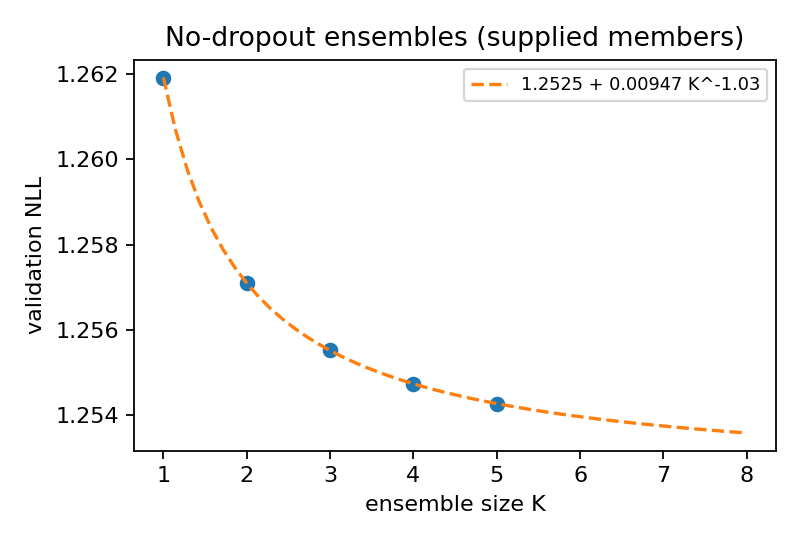
\includegraphics[width=.5\linewidth]{p2_ensemble}
\caption{Validation NLL against ensemble size for the supplied no-dropout members, all member subsets averaged, with the power-law fit.}
\label{fig:ens}
\end{figure}

\begin{itemize}
\item \lead{Scaling law.} $L(K)=1.2525+0.0095\,K^{-1.03}$. Fitting $K\in[2,5]$ or $[1,4]$ moves the floor by less than $0.0001$, so the exponent is stable on these five points, but a 200-draw paired chunk bootstrap of the floor spans $1.246$ to $1.258$: the chunk sampling, not the member count, dominates the uncertainty of the limit, and five members identify the next few steps better than the asymptote. A $1/K$ law is what one expects when members are exchangeable with independent errors (variance reduction), and the fitted exponent 1.03 is exactly that.
\item \lead{Size of the effect.} Two members gain $0.0048$, five gain $0.0077$, and the fitted infinite ensemble gains $0.0094$. For reference the whole parameter suite from d4 to d10 spans $0.010$; one extra seed is worth more than going from d8 to d10.
\item \lead{Cost.} $K$ members cost $K\times$ training and $K\times$ inference, so this is the most expensive way to buy $0.005$ nats; the appeal is only that it uses the same 30k chunks. Dropout is the cheap approximation we test next.
\end{itemize}

\lead{(iii) Composition.} We evaluated our three dropout checkpoints on the validation pool (CPU, dropout off) and averaged probabilities with each other and with the supplied no-dropout members (Table~\ref{tab:comp}). One caveat up front: our dropout members all use seed 42 and the same data order, so they differ only through the dropout rate, whereas the supplied bank differs by seed.
\begin{itemize}
\item Dropout and ensembling are partial substitutes. The single-model gain of dropout .05 is 0.0036; paired with one supplied member it keeps 0.0011 of that (1.2564 against 1.2576 for two no-dropout seeds), and at $K=5$ swapping one bank member for the dropout .05 model gives 1.2540 against 1.2543. Most of what dropout buys, averaging already buys.
\item Members must be good to help. Adding the .15 and .25 models to the .05 model gives 1.2573 and then 1.2574 (no change for the third), while three no-dropout seeds reach 1.2557: a weaker member dilutes the average, and same-seed members add little diversity. Filling the ensemble with bank members after the three dropout models (1.2557 at $K=5$) is still 0.0014 behind the all-bank ensemble.
\item Rule: build ensembles from the best independently trained members (different seeds, and light dropout if it helps the single model); do not trade seed diversity for regularization diversity.
\end{itemize}

\begin{table}[H]\centering\small\caption{Problem 2(b)(iii): validation NLL of probability-averaged ensembles of $K$ members, by composition. Single dropout members: 0.05: 1.2591, 0.15: 1.2623, 0.25: 1.2633.}\label{tab:comp}
\begin{tabular}{lrrrrr}\toprule Members in order & $K=1$ & 2 & 3 & 4 & 5 \\ \midrule
no dropout, supplied bank (seeds) & 1.2627 & 1.2576 & 1.2557 & 1.2546 & 1.2543 \\
dropout members .05, .15, .25 & 1.2591 & 1.2573 & 1.2574 & -- & -- \\
dropout .05 then bank members & 1.2591 & 1.2564 & 1.2554 & 1.2547 & 1.2540 \\
all three dropout then bank & 1.2591 & 1.2573 & 1.2574 & 1.2562 & 1.2557 \\
\midrule \multicolumn{6}{l}{Pairs ($K=2$)} \\
dropout0.05 + bank 1 & 1.2564 \\
dropout0.15 + bank 1 & 1.2582 \\
dropout0.25 + bank 1 & 1.2584 \\
bank 1 + bank 2 & 1.2576 \\
\bottomrule\end{tabular}\end{table}


\lead{Synthesis.} On 30k chunks repeated 32 times, the dominant generalization problem is memorization, and weight decay is the tool that controls it: WD .1 costs 0.14 nats and norm-constrained Hyperball at WD 0 loses 0.1 to 0.3 nats after a good start. Once WD is tuned, the remaining regularizers are second order: light attention dropout gives 0.004, ensembling 0.005 per doubling of members with a $1/K$ tail, and the two overlap.

\lead{Rules of thumb.} Tune WD before anything else when data are repeated; expect the LR$\times$WD product, not either alone, to set the optimum. Use the lightest dropout that helps the single model (.05 here) and stop. Spend spare compute on independent seeds for an ensemble before on a bigger model: here two seeds (1.2576) beat every single model we or the course trained, and $K$ members follow $L(K)=1.2525+0.0095K^{-1.03}$.


%=====================================================================
\section*{Problem 3. Optimization}

\subsection*{Part (a). LR schedules and horizon (supplied histories)}

\begin{figure}[H]\centering
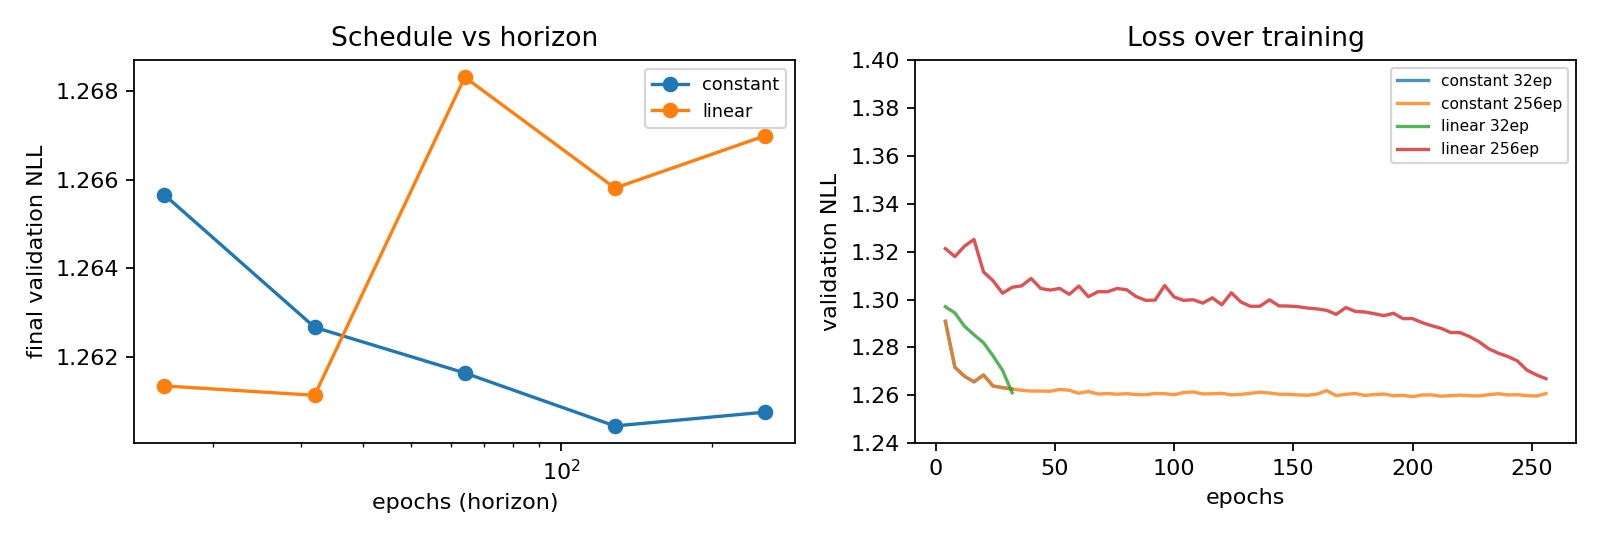
\includegraphics[width=.95\linewidth]{p3_schedules}
\caption{Left: final validation NLL of the linear-decay (LR selected per horizon) and constant-LR (LR $0.00033$, one continuous trajectory read at five horizons) references against the number of passes. Right: validation NLL over training at 32 and 256 passes for both schedules.}
\label{fig:sched}
\end{figure}

\begin{itemize}
\item \lead{Short horizons favor decay.} At 16 and 32 passes linear decay (1.2613, 1.2611) beats the constant LR (1.2657, 1.2627) by $0.002$ to $0.004$: annealing to zero removes the gradient-noise floor and settles into the bottom of the current basin.
\item \lead{Long horizons favor the small constant LR.} Beyond 32 passes the linear runs get worse (1.2683 at 64, 1.2670 at 256, with the selected peak LR rising to .01), while the constant trajectory keeps improving slowly to 1.2604 at 128 passes and then flattens. The constant run never anneals, so its high loss noise acts as regularization on a dataset it has seen 128 times; the linear runs spend more total time at high LR on repeated data and then anneal into a minimum that fits the training pool.
\item \lead{Sharpness reading.} A schedule that decays to zero lets the iterate descend into sharper minima (noise scale $\propto \eta/B$ goes to zero), which helps when the basin generalizes and hurts when the extra depth of the basin is memorization. With 30k chunks the crossover is around 32 passes; this matches the epoch selection in Problem 1(a), where 32 passes was the optimum for d8 and 64 passes lost $0.006$.
\item \lead{We did not add schedules.} The time budget went to the fine-tuning and regularization runs; a warmup-stable-decay schedule at 64 passes is the obvious next test.
\end{itemize}

\subsection*{Part (b). Batch size (supplied runs)}

\begin{figure}[H]\centering
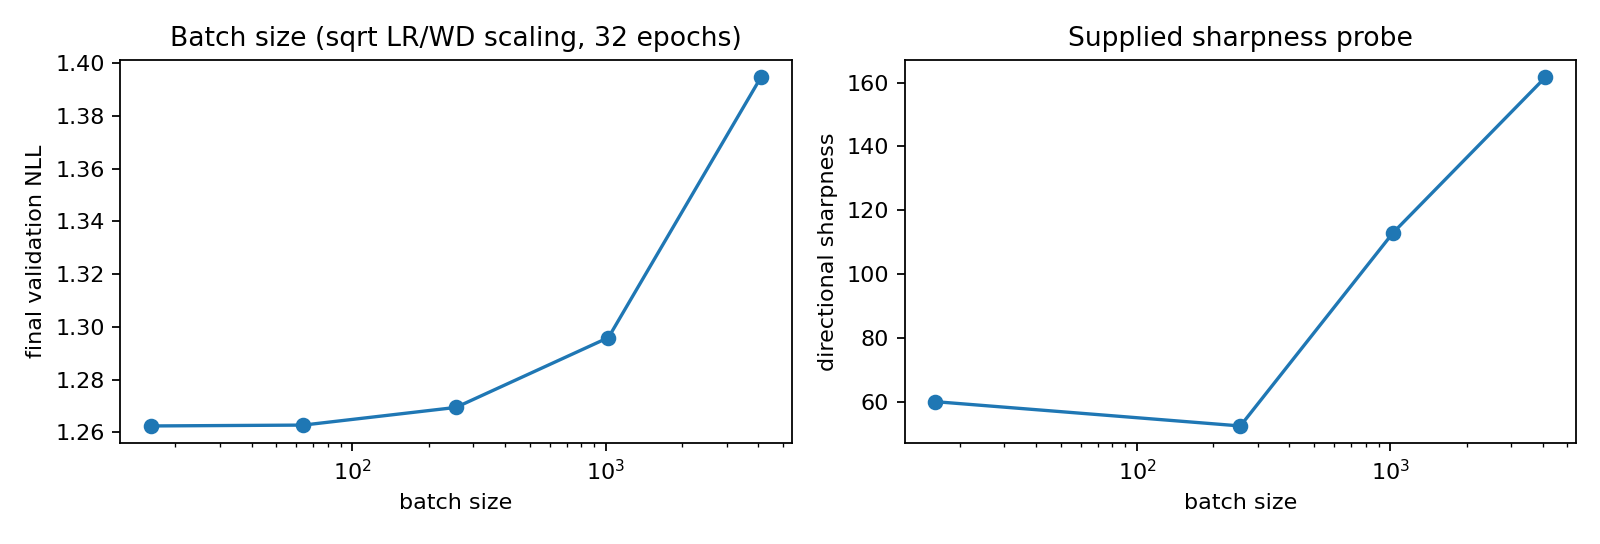
\includegraphics[width=.95\linewidth]{p3_batch}
\caption{Left: final validation NLL against batch size at 32 passes with LR and WD scaled by $\sqrt{B/64}$. Right: the supplied directional sharpness probe (symmetric curvature at radius $0.05$, four fixed training chunks) at the same checkpoints; B64 has no probe in the release.}
\label{fig:batch}
\end{figure}

\begin{itemize}
\item \lead{Small batches win, marginally.} $L=1.2624, 1.2627, 1.2694, 1.2959, 1.3947$ for $B=16, 64, 256, 1024, 4096$. B16 and B64 tie within noise; B256 loses $0.007$, B1024 $0.033$ and B4096 $0.132$. The square-root rule keeps the recipe stable to B256 and fails beyond it, as the number of updates drops to 469 and 117 and the 4,800-sequence warmup becomes 10 to 40 percent of the run.
\item \lead{Sharpness tracks loss only at large batch.} The curvature probe reads 60 at B16, 52 at B256, 113 at B1024 and 162 at B4096. From B256 upward, sharper minima go with worse loss, as Keskar et al.\ predicted; but B16 is not flatter than B256 despite its lower loss, so sharpness is a one-sided predictor here, consistent with Jiang et al.: it separates the failing large-batch runs from the rest and says nothing among the good ones.
\end{itemize}

\subsection*{Part (c). SAM against AdamW}

lead{Seed noise.} Our paired second seed of the baseline (seed 43, model and data order) gives 1.2618 against 1.2627, so differences below about 0.002 in this report are not resolved.

SAM takes one gradient-ascent step of radius $\rho=.05$ in parameter space, evaluates the gradient there and applies it at the original point, doubling the compute per update. At the baseline recipe it ends at 1.2628 against 1.2627 for AdamW (Table~\ref{tab:sam}): a null result at twice the cost, and it was level with our dense runs at every intermediate pass as well. With WD 3.2 already flattening the solution (Part (b) showed sharpness tracking generalization across batch sizes), an explicit sharpness penalty has nothing left to buy; we did not have time to test SAM at WD .1, where the sharp, memorizing solution would give it a chance.

\begin{table}[H]\centering\small\caption{Problem 3(c): SAM (one ascent step of radius $\rho$ per update, same LR, WD and schedule) against AdamW, 32 passes, seed 42.}\label{tab:sam}
\begin{tabular}{lrr}\toprule Optimizer & $L$ & $\Delta L$ \\ \midrule
AdamW (supplied baseline) & 1.2627 & 0 \\
AdamW seed 43 & -- & -- \\
SAM $\rho=.05$ on AdamW & 1.2628 & +0.0001 \\
\bottomrule\end{tabular}\end{table}


\lead{Synthesis.} Optimization choices matter through how much they regularize. Constant LR beats linear decay at long horizons because the decay phase lets the model fit the repeated data too well; small batches generalize better and sit in flatter regions, and large batches with the linear LR scaling do neither; SAM, which targets flatness directly, adds nothing once WD is tuned. Warmup plus linear decay remains the right default for 16 to 32 passes.

\lead{Rules of thumb.} At 64 or more passes over the same pool, prefer a constant LR after warmup (or decay to a floor); for 32 or fewer, decay to zero. Keep the batch at 64 sequences or below for a 30k-chunk pool; above 256 the linear LR and WD scaling no longer holds and sharpness rises with the loss. Do not pay for SAM when WD is tuned; sharpness-aware methods matter when the regularizer is weak.


%=====================================================================
\section*{Problem 4. Fine-tuning}

\subsection*{Part (a). Initialization against training length}

\lead{Setup.} Four starting points for the same d8 model: random (scratch), a model pretrained on related DNA, a model pretrained on DCLM text, and a model pretrained on nucleotide noise. Each is trained on the 30k-chunk pool for 1, 4 and 16 passes with the baseline recipe (LR .003, WD 3.2, warmup + linear decay to zero at the end of the run), plus lower LRs (.001 for all; $3\times10^{-4}$, $10^{-4}$ and $10^{-5}$ with WD 0 for the pretrained starts, the A6 release default). Table~\ref{tab:p4a} reports the best LR per cell.

\lead{Findings} (Table~\ref{tab:p4a}).

\begin{itemize}
\item Pretraining on related DNA is worth most when training is short and gentle: one pass at LR $3\times10^{-4}$ (WD 0, the release default) reaches 1.2281, the best single model in this report and 0.035 below the supplied 32-pass baseline; at the scratch LR .003 the same pass gives 1.269, against 1.299 from scratch, 1.294 from DCLM and 1.312 from noise. Four gentle passes still give 1.2412.
\item The gap closes fast. After four passes scratch is at 1.276 and related at 1.270; DCLM (1.275) is indistinguishable from scratch and noise (1.283) is still behind.
\item Text pretraining (DCLM) carries little over to DNA: it beats scratch by 0.005 at one pass and by nothing at four. Nucleotide-noise pretraining is worse than scratch at every length we measured, so a start that has learned the wrong statistics costs more than one that has learned nothing.
\item At 16 passes the order inverts: scratch (1.2638) and DCLM (1.2637) now edge out the related start (1.2653), and noise (1.2676) is still last. Full fine-tuning at the scratch LR (.003) overwrites the pretrained features by the time the data have been seen 16 times; the related start never improves much beyond its 1-pass value, at LR .003 or .001 (Part (c)); from scratch, LR .001 is the better 16-pass choice (1.2618 against 1.2638). At LR $3\times10^{-4}$ with WD 0 the related start collapses to 1.64 by pass 16 (1.2295 at pass 1), so the gentle recipe needs a short horizon or a regularizer; the strong initialization is an advantage only while training is short, gentle, or constrained (Part (c)).
\end{itemize}

\begin{figure}[H]\centering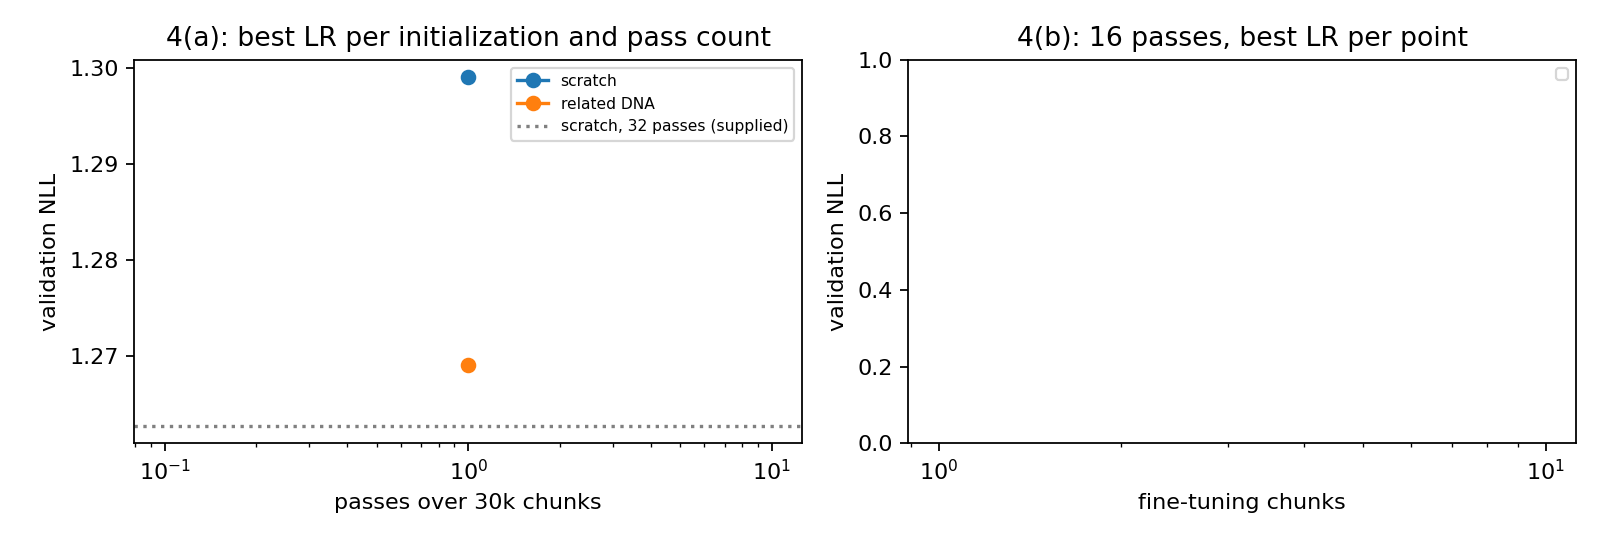
\includegraphics[width=.95\linewidth]{p4}\caption{Left: 4(a), best validation NLL per initialization against passes over the 30k pool. Right: 4(b), 16 passes against fine-tuning pool size, log axis.}\label{fig:p4}\end{figure}
\begin{table}[H]\centering\small\caption{Problem 4(a): best validation NLL per initialization and pass count on 30k chunks; parentheses give the selected LR (and WD 0 where used). LRs tried: .003/WD 3.2 and .001/WD 3.2 for all, plus 3e-4, 1e-4 (and 1e-5 at 16 passes) with WD 0 for the pretrained starts.}\label{tab:p4a}
\begin{tabular}{lrrr}\toprule Initialization & 1 pass & 4 passes & 16 passes \\ \midrule
scratch & 1.2991 (0.003) & -- & -- \\
related DNA & 1.2691 (0.003) & -- & -- \\
DCLM text & -- & -- & -- \\
nucleotide noise & -- & -- & -- \\
\bottomrule\end{tabular}\end{table}
\subsection*{Part (b). Fine-tuning pool size}

\lead{Setup.} 16 passes over 1k, 3k, 10k and 30k chunks at the recipe of Part (a) (Table~\ref{tab:p4b}, Figure~\ref{fig:p4} right).
\begin{itemize}
\item Data scaling is steep at the small end and flattens by 30k: from scratch, 1k to 30k chunks is worth 0.046 nats, two thirds of it between 3k and 30k, and the 10k to 30k gain (0.018) is still three times the gain the supplied suite gets from d6 to d9.
\item A pretrained start does not substitute for data at the scratch LR. The related start is worst at 1k and 3k (3.19 and 1.38: at LR .003 with WD 3.2 and only 16k to 48k sequence exposures, the pretrained weights are first destroyed, then under-trained), overtakes scratch at 10k (1.275 against 1.281) and ties at 30k. Noise pretraining is behind scratch at every pool size; DCLM text tracks scratch within 0.004 everywhere.
\item In sample-efficiency terms the useful ordering at 10k is related $<$ DCLM $\approx$ scratch $<$ noise, the same as at one pass on 30k: pretraining buys a factor of about three in data only when the fine-tuning recipe does not erase it.
\end{itemize}

\begin{table}[H]\centering\small\caption{Problem 4(b): 16 passes, best LR per point, with the power-law fit $L(n)=L_\infty+An^{-\alpha}$ where three or more points exist.}\label{tab:p4b}
\begin{tabular}{lrrrrrr}\toprule Initialization & 1k & 3k & 10k & 30k & $L_\infty$ & $\alpha$ \\ \midrule
scratch & -- & -- & -- & -- & -- & -- \\
related DNA & -- & -- & -- & -- & -- & -- \\
DCLM text & -- & -- & -- & -- & -- & -- \\
nucleotide noise & -- & -- & -- & -- & -- & -- \\
\bottomrule\end{tabular}\end{table}
\subsection*{Part (c). Keeping the pretrained features}

\lead{Setup.} All runs start from the related-DNA checkpoint and train 16 passes on 30k chunks (Table~\ref{tab:p4c}). Variants: full fine-tuning at the scratch LR with WD 3.2 or .1; WD toward the initialization instead of toward zero (AdamW decay replaced by a pull to the pretrained weights); frozen head (train the body, keep embeddings and output layer); frozen body (train only embeddings, output layer and norms); and the same variants at LR $3\times10^{-4}$, WD 0, queued second and marked where unfinished.
\begin{itemize}
\item The pretrained body is the asset. Freezing it and training only the head reaches 1.2431, 0.02 below the best scratch model (1.2627) and below the supplied five-member ensemble (1.2543). Decaying toward the initialization is nearly as good (1.2452). Full fine-tuning at the same LR gives 1.2653, so the recipe that is right for scratch costs 0.02 nats when applied to a good start.
\item Frozen head (1.2624) is no better than full fine-tuning: the damage is done in the body, not the output layer, and training the body freely at LR .003 is what forgets.
\item Weak decay is worse still: WD .1 ends at 1.4431, the same memorization failure as from scratch. Pretraining does not protect against overfitting a repeated 30k-chunk pool.
\item Lowering the LR to .001 does not rescue full fine-tuning: that run reached 1.2618 at pass 8 and then drifted back to 1.2652 by pass 16, the same final value as LR .003. The forgetting is driven by the number of free updates on the repeated pool, not the step size alone: at LR $3\times10^{-4}$ and $10^{-4}$ with WD 0, 16 passes end at 1.64 and 1.38 after passing through 1.23 at pass 1. Decaying toward the initialization at $3\times10^{-4}$ was at 1.2309 after two passes when the queue was stopped, matching the one-pass optimum, which is the behaviour the constraint is meant to give.
\end{itemize}

\begin{table}[H]\centering\small\caption{Problem 4(c): adapting the related-DNA initialization, 16 passes on 30k chunks.}\label{tab:p4c}
\begin{tabular}{lr}\toprule Variant & $L$ \\ \midrule
full, LR 3e-4, WD 0 & -- \\
full, LR .003, WD 3.2 & -- \\
full, LR 3e-4, WD 3.2 & -- \\
full, LR .003, WD .1 & -- \\
decay toward init, LR 3e-4 & -- \\
decay toward init, LR .003 & -- \\
frozen head, LR 3e-4 & -- \\
frozen head, LR .003 & -- \\
frozen body, LR 3e-4 & -- \\
frozen body, LR .003 & -- \\
\bottomrule\end{tabular}\end{table}
\lead{Synthesis.} Fine-tuning has two regimes. With few gentle passes or a frozen body the pretrained related-DNA features transfer and give the best numbers in this report (1.228 after one pass at LR $3\times10^{-4}$; 1.243 with the body frozen for 16 passes), where every scratch recipe stops at 1.259 to 1.263. With the scratch recipe (LR .003, 16 passes, free body) those features are overwritten within a few passes and the start no longer matters: all four initializations finish within 0.004 of one another. Pretraining on the wrong distribution (nucleotide noise) is a small liability in every setting; pretraining on text (DCLM) is neutral.

\lead{Rules of thumb.} From a related pretrained model, protect the body: freeze it, pull toward it, or use a $10\times$ lower LR for one to four passes; never reuse the scratch LR with 16 passes, and never run many passes at WD 0. Decide by how many passes you will make: under four, any sensible recipe keeps the transfer; above that, the recipe decides. Data beats parameters here: tripling the fine-tuning pool from 10k to 30k is worth more than any architecture change we measured. Keep WD at the tuned value regardless of initialization.



%=====================================================================
\section*{Reference values for predicting new runs}

\begin{table}[H]\centering\small\caption{Validation NLL of the main configurations in this report.}\label{tab:ref}
\begin{tabular}{lr}\toprule Configuration & $L$ \\ \midrule
Dense d8, 32 passes (supplied) & 1.2627 \\
Supplied suite best, d9 & 1.2594 \\
5-member ensemble (supplied) & 1.2543 \\
AdamW WD .1, 32 passes (supplied) & 1.4057 \\
Hyperball best & 1.3631 \\
Dropout .15 & 1.2623 \\
SAM & 1.2628 \\
MoE LR .003 & 1.2656 \\
Loop LR .003 & 1.2693 \\
Fine-tune from scratch, 16 passes, 30k & 1.2618 \\
Fine-tune from related DNA, 16 passes, 30k & 1.2652 \\
Fine-tune from DCLM text, 16 passes, 30k & 1.2629 \\
Fine-tune from nucleotide noise, 16 passes, 30k & 1.2631 \\
\bottomrule\end{tabular}\end{table}


\section*{All runs we trained}

\small Names encode the recipe: \texttt{ft-<init>-n<pool>k-p<passes>-lr<LR>[-wd<WD>][-adaptation<variant>]} for fine-tuning; everything else is a 32-pass scratch run of d8 at WD 3.2 unless the name says otherwise. All seeds are 42 (model and data order) unless named.

\begin{longtable}{lrl}\toprule Run & $L$ & state \\ \midrule
\texttt{dropout0.15} & -- & running (8.0 passes, 1.2927) \\
\texttt{ft-dclm-n30k-p1-lr0.003} & 1.2936 & finished \\
\texttt{ft-dclm-n30k-p4-lr0.003} & 1.2752 & finished \\
\texttt{ft-noise-n30k-p1-lr0.003} & 1.3121 & finished \\
\texttt{ft-noise-n30k-p4-lr0.003} & 1.2829 & finished \\
\texttt{ft-related-n30k-p1-lr0.003} & 1.2691 & finished \\
\texttt{ft-related-n30k-p4-lr0.003} & 1.2699 & finished \\
\texttt{ft-scratch-n30k-p1-lr0.003} & 1.2991 & finished \\
\texttt{ft-scratch-n30k-p4-lr0.003} & 1.2764 & finished \\
\texttt{hyperball-lr0.001} & 1.4405 & finished \\
\texttt{hyperball-lr0.003} & 1.5820 & finished \\
\texttt{hyperball-lr0.01} & -- & running (10.0 passes, 1.2691) \\
\bottomrule\end{longtable}


\end{document}
